\documentclass[12pt]{beamer}
%\documentclass[20pt,handout]{beamer}
\usetheme{Darmstadt}
\usepackage{graphicx}
%\usepackage[german]{babel}
\usepackage{ngerman}
\usepackage[T1]{fontenc}
\usepackage[utf8]{inputenc}
\usepackage{tikz}
\setbeamertemplate{footline}[frame number]

\newcommand{\cc}[1]{\includegraphics[height=4mm]{img/#1.png}\hspace{1mm}}
\usepackage{ifthen}
\newcommand{\license}[2][]{\\#2\ifthenelse{\equal{#1}{}}{}{\\\scriptsize\url{#1}}}
\usepackage{textcomp}
\usepackage{hyperref}

\pgfdeclareimage[height=.6cm]{c3d2logo}{./img/c3d2.pdf}


\pgfdeclarelayer{foreground}
\pgfsetlayers{main,foreground}
\logo{\pgfputat{\pgfxy(-1,0)}{\pgfbox[center,base]{\pgfuseimage{c3d2logo}}}}


\title{Smartphones und Datenschutz}
\author{\small Stephan Thamm und Paul Schwanse\\\large Chaos Computer Club Dresden}
\date{18.03.2015}

\begin{document}
\maketitle


\section{Einleitung}
\subsection{}

\begin{frame}
    \frametitle{Chaos Computer Club}
    \begin{center}
	
\includegraphics[height=0.2\textheight]{img/chaosknoten.png}
    \end{center}	
    \begin{itemize}
      \item<1-> Verein wurde 1981 gegr"undet (\url{https://ccc.de})          
      \item<2-> Aktuell ca. 4500 Mitglieder
      \item<3-> Betreibt u.a. "Offentlichkeitsarbeit und Politikberatung      
    \end{itemize}
\end{frame}

\begin{frame}
  \frametitle{Chaos Computer Club}
  \begin{figure}
    
\includegraphics[height=0.7\textheight]{img/fingerabdruck.jpg}
  \end{figure}
\end{frame}

\begin{frame}
  \frametitle{Chaos Computer Club}
  \begin{figure}
    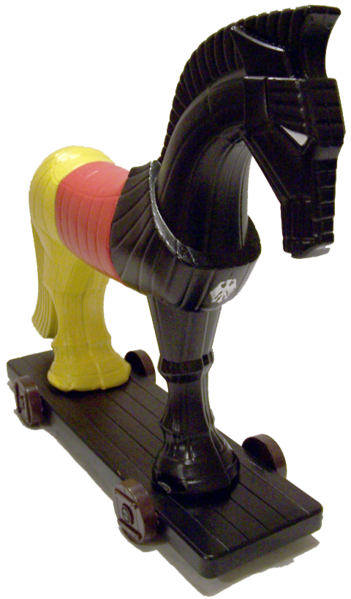
\includegraphics[height=0.7\textheight]{img/trojaner.png}
  \end{figure}
\end{frame}

\begin{frame}
    \frametitle{Chaos Computer Club}
    \begin{center}
	
\includegraphics[height=0.1\textheight]{img/c3d2_logo.png}
    \end{center}
    \begin{itemize}
      \item<1-> Chaos Computer Club Dresden (\url{https://c3d2.de})          
      \item<2-> Datenspuren: Oktober 2015 (\url{https://datenspuren.de})
      \item<3-> Podcasts (\url{https://c3d2.de/radio.html})
      \item<4-> Chaos macht Schule (\url{https://c3d2.de/schule.html})
    \end{itemize}
\end{frame}

\begin{frame}
    \frametitle{Fragerunde}
    \begin{itemize}
	    \item<2-> Wieviele von ihnen nutzen aktive ein Smartphone?
	    \item<3-> Wie viele ihrer Schüler nutzen aktiv ein Smartphone?
	    \item<4-> Wie viele ihrer Schüler sind mit den Einstellmöglichkeiten ihres Smartphones vertraut?
	    \item<5-> Wie viele von ihnen sind mit den Einstellmöglichkeiten ihres Smartphones vertraut?
    \end{itemize}
\end{frame}

\section{Ebenen beim Smartphone}
\subsection{Hardware}
\begin{frame}
	\frametitle{Hardware}
	\begin{itemize}
		\item<2-> WLAN
		\item<3-> GPS
		\item<4-> Bewegungssensoren
		\item<5-> Kamera, Mikrofon
		\item<6-> Telefoniefunktion
		\item<7-> Erweiterungsslots
	\end{itemize}
\end{frame}

\subsection{Betriebssystem}
\begin{frame}
	\frametitle{Betriebssystem}
	\begin{itemize}
		\item<2-> Google-Konto / Apple ID
		\item<3-> App Stores
		\item<4-> Zugriffsrechtemanagement
		\item<5-> Updates
	\end{itemize}
\end{frame}

\subsubsection{App Stores}
\begin{frame}
	\frametitle{App Stores}
	\begin{itemize}
		\item<2-> Zugang zum App Store wird kontrolliert
		\item<3-> Hoheit darüber, welche Software installiert werden kann
		\item<4-> Datenschutz Level wird kontrolliert
		\item<5-> Updateproblem
		\item<6-> Verknüpfung mit Cloud Diensten
	\end{itemize}
\end{frame}

\subsubsection{Apps}
\begin{frame}
	\frametitle{Apps}
	\begin{itemize}
		\item<2-> Zugriff auf ...
		\begin{itemize}
			\item<3-> persönliche Daten
			\item<4-> PhoneID
			\item<5-> Sensoren
			\item<6-> Kamera, Mikrofon
			\item<7-> Netzwerk
		\end{itemize}
		\item<8-> Durch Benutzung der App entstehende Privatsphärenprobleme
	\end{itemize}
\end{frame}

\section{App Permission Restrictions}
\subsection{App Permission Restrictions}
\begin{frame}
	\frametitle{App Permission Restrictions}
	\begin{itemize}
		\item<2-> Regeln Zugriffsrechte einer App
		\item<3-> Wettbewerb um Datenschutz wird nicht gefördert
		\item<4-> Wo findet man, welche Rechte eine App braucht?
	\end{itemize}
\end{frame}

\subsection{Mitmach Teil}
\begin{frame}
	\frametitle{Ratespiel}
	\begin{itemize}
		\item<2-> Behältnis mit Zetteln mit Zugriffsrechten
		\item<3-> Auf Zettel stehen Zugriffsrechte, Rückseite hat Nummer
		\item<4-> Privatsphärenverletztendes Szenario kreieren
		\item<5-> Raten, um welche App es sich gehandelt hat
		\item<6-> Sensibilisiert die Schüler, wie man ihre Privatsphäre ausspionieren kann
		\item<7-> Szenarien sollen kreativ sein
	\end{itemize}
\end{frame}

\section{Alternative App Stores}
\subsection{Alternative App Stores}
\begin{frame}
	\frametitle{Alternative App Stores}
	\begin{itemize}
		\item<2-> Entwickler haben anderen Fokus
		\item<3-> mehr Datenschutz
		\item<4-> weniger Kommerz
		\item<5-> viele Probleme mit Community gelöst
		\item<6-> Spiele, Sensoren auslesen, \ldots
	\end{itemize}
\end{frame}
\subsection{Alternative Android ROMs}
\begin{frame}
	\frametitle{Alternative Android ROMs}
	\begin{itemize}
		\item<2-> basiert auf quelloffenen Teilen von Android
		\item<3-> meistens fügen Hersteller weitere Software hinzu
		\item<4-> alternative ROMs auf Datenschutz fixiert als "`Verkaufsargument"'
		\item<5-> Telefon muss gerootet werden, Wissen, Garantie
	\end{itemize}
\end{frame}

\begin{frame}
	\frametitle{Liste an Android ROMs, anderen OS}
	\begin{itemize}
		\item<2-> Cyanogenmod, \ldots
		\item<3-> Firefox OS
		\item<4-> Sailfish OS/Jolla
		\item<5-> Ubuntu
	\end{itemize}
\end{frame}
\end{document}
